Manifold learning... showcase how this would solve the swiss roll

\subsection{Manifolds} 

This concept is significantly more difficult to get a hold of.
Significant breakthroughs \cite{ma2012manifold} in this field were accomplished in the year 2000 in the significant and commonly cited paper \emph{A global geometric framework for nonlinear dimensionality reduction}. \cite{tenenbaum2000global}
To understand the basic idea, we will demonstrate its behaviour to get an idea of the problem using the popular swiss roll data set pictured in figure \ref{fig:swissrollfull}.


\noindent
\begin{minipage}[c]{0.4\linewidth}
%
\vspace*{6mm}
\begin{center}
	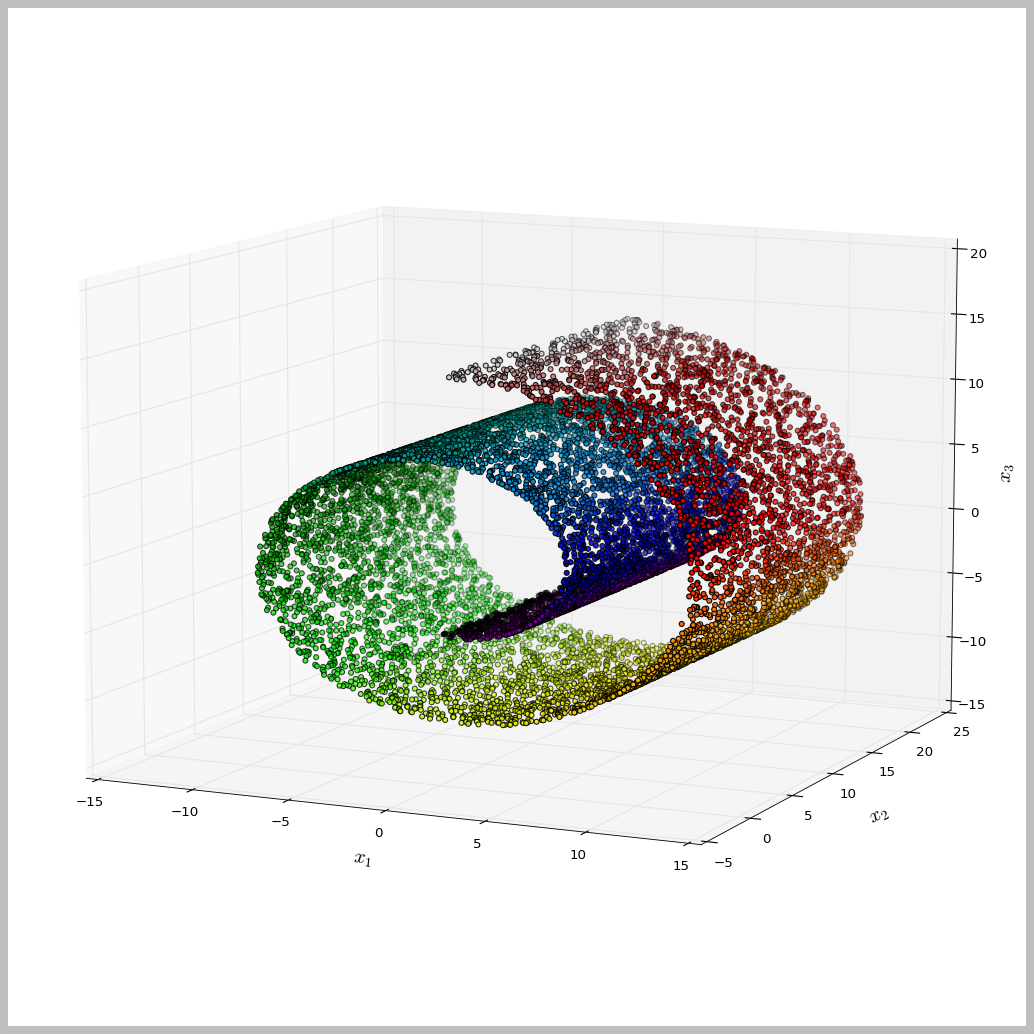
\includegraphics[width=0.9\textwidth]{external_content/graphs/swiss_roll.png}
	\captionsetup{justification=centering,type=htypei}
	\captionof{figure}{Swiss Roll generated from scikit-learn \cite{scikit-learn}}
	\label{fig:swissrollfull}
\end{center}
%
\end{minipage}\hfill%
\begin{minipage}[c]{0.55\linewidth}
Before demystifying this problem, we will then dive into various methods how to bend and twist high-dimensional data into lower-dimensional spaces.

Our goal is to avoid confusing projections such as shown in figure \ref{fig:swissrollprojection}:

\begin{center}
	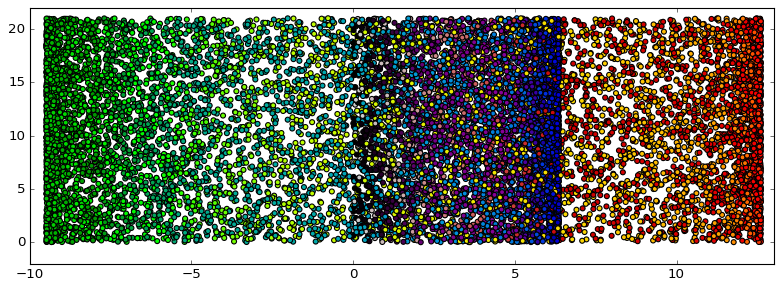
\includegraphics[width=0.8\textwidth]{external_content/graphs/swiss_roll-projection.png}
	\captionsetup{justification=centering,type=htypei}
	\captionof{figure}{Representation in 2D\\ of a projected swiss role}
	\label{fig:swissrollprojection}
\end{center}
\end{minipage}%

